\documentclass[11pt,xcolor={dvipsnames},aspectratio=159,hyperref={pdftex,pdfpagemode=UseNone,hidelinks,pdfdisplaydoctitle=true},usepdftitle=false]{beamer}
\usepackage{presentation}[aspectratio=169]
\usepackage{math}
\usepackage{mathtools}
\usepackage{mleftright}
\usepackage{algorithm}% http://ctan.org/pkg/algorithms
\usepackage{algpseudocode}% http://ctan.org/pkg/algorithmicx
\hypersetup{
    colorlinks=magenta,
    linkcolor=magenta,
    filecolor=magenta,      
    urlcolor=magenta,
    }
% Enter title of presentation PDF:
\hypersetup{pdftitle={Function Approximation}}
% Enter link to PDF file with figures:


\begin{document}
% Enter presentation title:
\title{Function Approximation}
\subtitle{Quantitative Economics 2024}
% Enter presentation information:

% Enter presentation authors:
\author{Piotr Żoch}%
% Enter presentation location and date (optional; comment line if not needed):
\frame{\titlepage}

% Fill out content of presentation:
\begin{frame}{What is it?}   
    \alg{Goal}: approximate a complicated function $f: \R^n \rightarrow \R$ by a simpler function $\hat{f}: \R^n \rightarrow \R$.
\begin{itemize}
    \item We know $f$ only at a finite number of points and we want to approximate it at other points $x$.
    \item $f$ is too complicated to work with directly (e.g. non-analytic) and we need to represent on a computer.
\end{itemize}

I will talk only about the \al{most basic} ideas. 

\end{frame}
\begin{frame}{Function approximation}   
\begin{itemize}
    \item  What data should be produced and used?
    \item  What family of “simpler” functions should be used?
    \item  What notion of approximation do we use?
    \item  How good can the approximation be?
    \item  How simple can a good approximation be?
\end{itemize}

Notice \alb{similarities} and \alr{differences} between function approximation and statistical regression.

\end{frame}

\begin{frame}{Notation}   
    \begin{itemize} 
      \item Today we will focus on continuous functions $f: \R^n \rightarrow \R$.
      \item  We can represent every continuous function in a particular function space
      by a linear combination of \al{basis functions}.
      \item  Analogy: Every vector in a vector space $V$ can be represented by a linear combination of basis vectors.
     \end{itemize}
\end{frame}

\begin{frame}{Notation}   
    \begin{itemize} 
      \item Let $F$ by the space of continuous real-valued functions with domain $X\subset\R^n$.
      \item Define the \alg{inner product} of two functions $f, g \in F$ as 
      \begin{align*}
            \langle f, g \rangle = \int_{X} f\of{x} g\of{x} w\of{x} dx
        \end{align*}
        where $f,g,w \in F$, $w$ is a \alg{weighting function}.
        \item $\bc{F, \langle \cdot, \cdot \rangle}$ is an inner product space.
        \item We want to approximate a \al{known} function $f : X \rightarrow \R$ in $\bc{F, \langle \cdot, \cdot \rangle}$.
        
       \end{itemize}
\end{frame}

\begin{frame}{Notation}   
    \begin{itemize} 
      \item Let $\hat{f}\of{\cdot,\beta}$ be a parametric approximation of $f$. We have 
      \begin{align*}
            \hat{f}\of{x,\beta} = \sum_{j=0}^{J} \beta_j \phi_j\of{x}
      \end{align*}
        
        \begin{itemize}
                \item $\phi_j\of{x}$ are \alg{basis functions}. Write $\Phi_J = \bc{\phi_0, \phi_1, \ldots, \phi_{J}}$.
                \item $\beta = \bs{\beta_0,\beta_1,\ldots,\beta_{J}}$ is a vector of coefficients.
                \item $J$ is the order of interpolation.
            \end{itemize}    
      \item We want to find $\beta$ such that $\hat{f}\of{\cdot,\beta}$ is a "good" approximation of $f$.
      \item Define the residual function  $r\of{x,\beta} \coloneqq f\of{x} - \hat{f}\of{x,\beta}$. We want to make it small in some sense.
        \end{itemize}
      
\end{frame}




\begin{frame}
    \heading{Spectral methods}
    \end{frame}

    \begin{frame}{Spectral methods}
    \begin{itemize} 
        \item \al{Spectral methods}: basis functions are non-zero on the entire domain of $f$.
        \item Polynomial interpolation: basis functions are polynomials
        \item Fourier series: basis functions are sines and cosines
    \end{itemize}
        \end{frame}
    

\begin{frame}{Interpolation}   
    \begin{itemize} 
      \item Suppose we know $f$ at $N=J+1$ points $\bc{x_i}_{i=0}^{J}$. We call these points \alb{interpolation nodes}.
      \item Note: we have the \al{same number} of points as basis functions.
      \item Let $r_i$ be the residual at $x_i$. We have
      
      \begin{align*}
        \left[\begin{array}{c}
        r_0\\
        \vdots\\
        r_J\\
        \end{array}\right] & =\left[\begin{array}{c}
        f\of{x_0}\\
        \vdots \\
        f\of{x_0}\\
        \end{array}\right]-\left[\begin{array}{ccc}
        \phi_{0}\of{x_0} & \cdots & \phi_{J}\of{x_0}\\
        \vdots & \ddots & \vdots \\
        \phi_{0}\of{x_J} & \cdots & \phi_{J}\of{x_J}\\
        \end{array}\right]\left[\begin{array}{c}
        \beta_0 \\
        \vdots \\
        \beta_J \\
        \end{array}\right]
    \end{align*}
    \item Abuse notation and write it as \begin{align*}r = f - \Phi \beta\end{align*}.  
        \end{itemize}
      
\end{frame}

\begin{frame}{Interpolation} 
    \begin{itemize}
        \item The idea of \al{interpolation} is to find $\beta$ such that $r_i = 0$ for all $i$. 
        \item The unknowns are the coefficients $\beta$.
        \item This is equivalent to solving the linear system of equations 
        \begin{align*}
            \Phi \beta = f
        \end{align*}
        with an obvious solution $\beta = \Phi^{-1} f$.
    \end{itemize}
\end{frame}

\begin{frame}{Regression} 
    \begin{itemize}
        \item If we have more points than basis functions, $M>J+1$ we cannot interpolate. 
        \item We have to define a loss function $L\of{\cdot,r}$ and minimize it.
        \item If we use the squared loss function 
        \begin{align*}L\of{x,r} = \sum^M_{i=0} r\of{x_i,\beta}^2,\end{align*} we get the \al{least squares} problem with solution
        \begin{align*}
            \beta = \bp{\Phi^T \Phi}^{-1} \Phi^T f
        \end{align*}

    \end{itemize}
\end{frame}



\begin{frame}{Weierstrass theorem} 
    \begin{theorem}
        Let $f: \bs{a,b} \rightarrow \R$ be a continuous function. Then for every $\varepsilon > 0$ there exists a polynomial $p$ such that $$\sup_{x \in \bs{a,b}} \abs{f\of{x} - p\of{x}} \leq \varepsilon.$$
              \end{theorem}

        \begin{itemize}
        \item We can approximate any continuous function on a compact set by a \al{polynomial} as closely as we want.
        \end{itemize}
\end{frame}

\begin{frame}{Basis function choice} 
    \begin{itemize}
        \item Which basis functions should we use? 
        \item The most natural choice seems to be \al{monomials}: $\phi_j\of{x} = x^j$.
        \item Problem: consecutive monomials are very similar to each other -- does $x^{10}$ really add much to $x^{9}$?
        \item The resulting matrix $\Phi$ is a \alb{Vandermonde matrix}, which is \alr{ill-conditioned}.
    \end{itemize}
\end{frame}

\begin{frame}{Basis function choice} 
    \begin{itemize}
        \item If $\Phi$ looks like a diagonal matrix, then $\Phi^{-1}$ is easy to compute. 
        \item Intiuition: use basis functions that give us \al{different} information about $f$.
        \item \alg{Orthogonal polynomials} are a good choice: $\langle \phi_i, \phi_j \rangle = 0$ for $i\neq j$.
    \end{itemize}
\end{frame}

\begin{frame}{Orthogonal polynomials}
    \begin{itemize}
        \item For orthogonal polynomials, we have 
        \begin{align*}
            \beta_j = \int_{X} f\of{x} \phi_j\of{x} w\of{x} dx
        \end{align*}
        \item Intiuition: use basis functions that give us \al{different} information about $f$.
        \item \alg{Orthogonal polynomials} are a good choice: $\langle \phi_i, \phi_j \rangle = 0$ for $i\neq j$.
        \item Examples: Legendre, Chebyshev, Hermite, Laguerre, Jacobi polynomials.
    \end{itemize}
\end{frame}

\begin{frame}{Chebyshev polynomials}
    \begin{itemize}

        \item \al{Chebyshev polynomials} $T_n\of{x}: \bs{-1,1} \rightarrow \R$ are given by \begin{align*}
        T_0\of{x} &= 1 \\
        T_1\of{x} &= x \\
        T_{j+1}\of{x} &= 2xT_j\of{x} - T_{j-1}\of{x}
        \end{align*}
        \item Let $X = [-1,1]$ and $w\of{x} = \frac{1}{\sqrt{1-x^2}}$. We have 
        \begin{align*}
            \langle T_i, T_j \rangle = \int_{-1}^{1} T_i\of{x} T_j\of{x} \frac{1}{\sqrt{1-x^2}} dx = \begin{cases}
                0 & i\neq j \\
                \pi & i = j = 0 \\
                \frac{\pi}{2} & i = j \neq 0
            \end{cases}
        \end{align*}
    \end{itemize}
\end{frame}

\begin{frame}{Chebyshev polynomials}
    \centering
    \begin{figure}
        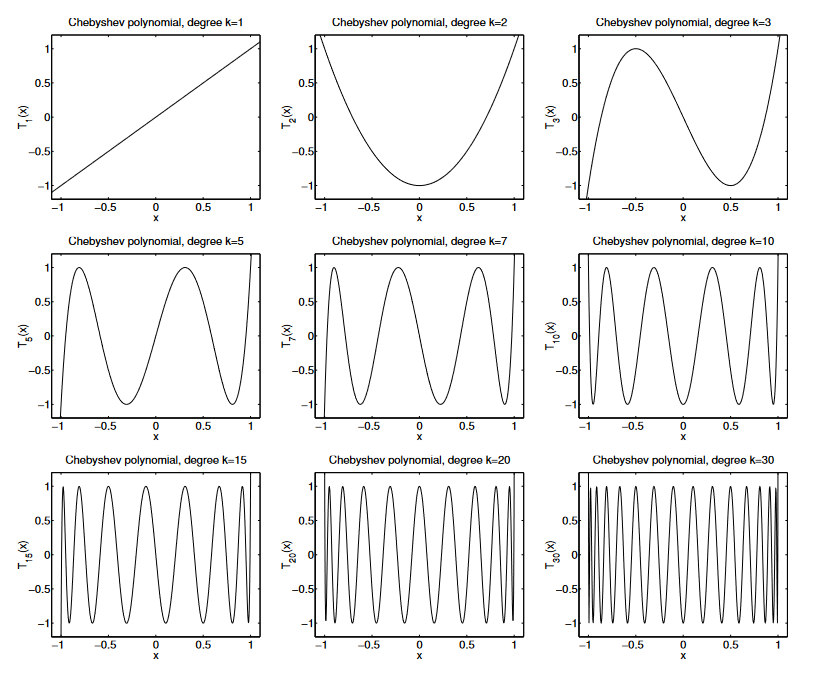
\includegraphics[width=0.55\textwidth]{chebyshev.png}
    \end{figure}
    \end{frame}

\begin{frame}{Chebyshev nodes}
    \begin{itemize}
        \item \alg{Orthogonality} is not the only nice property of Chebyshev polynomials.
        \item \al{Chebyshev nodes} are roots of Chebyshev polynomials on $[-1,1]$: 
        \begin{align*}
        x_i = \cos\of{\frac{2i-1}{2n}\pi} \quad \text{for} \quad i = 1,\ldots,n.
        \end{align*}
        It can be verified that $T_n$ equals 0 at these points.
        \item Chebyshev nodes are not equally spaced, they are \al{clustered} at the endpoints of the interval.
    \end{itemize}
\end{frame}

\begin{frame}{Chebyshev nodes}
    \begin{itemize}
        \item In practice we want to work on $\bs{a,b}$. We can use an affine transformation to get
        \begin{align*}
        x_i = \frac{1}{2} \bp{a+b} + \frac{1}{2} \bp{b-a} \cos\of{\frac{2i-1}{2n}\pi} \quad \text{for} \quad i = 1,\ldots,n.
        \end{align*}
    \end{itemize}
\end{frame}

\begin{frame}{Nodes choice}
    \begin{itemize}
        \item Why are these nodes useful?
        \item We know that at the interpolation nodes $x_i$ we have $r_i = 0$. 
        \item We want to make the residual as small as possible at other points $x$.
        \item A silly choice of nodes (e.g. equidistant) can lead to a large residual at other points, even with a high order of interpolation -- \al{Runge phenomenon}.
        \item \al{Minmax approximation}: polynomial approximation using Chebyshev nodes is very close to the polynomial approximation that minimizes the maximum absolute error on $\bs{-1,1}$.
    \end{itemize}
\end{frame}



\begin{frame}{Chebyshev regression}
    \begin{enumerate}

        \item Obtain $M\geq J + 1$ Chebyshev nodes $z_m \text{ for } m = 0,\ldots,M$ on $\bs{-1,1}$.
        \item Transform the nodes to $\bs{a,b}$: \begin{align*}
            x_m = \bp{z_m + 1}\frac{b-a}{2} \quad \text{for } m = 0,\ldots,M.
        \end{align*}
        \item Evaluate $f$ at $x_m$ to get $f_m$.
        \item Compute $\beta_j \text{ for } j = 0,\ldots,J$ using the least squares formula: 
        \begin{align*}
            \beta_j = \frac{\sum_{m=0}^M f_m T_j\of{z_m} }{\sum_{m=0}^M T_j\of{z_m}^2} \ \text{for } j = 0,\ldots,J.
        \end{align*}
        to get the approximation of $f\of{x} \text{ on } \bs{a,b}$ \begin{align*}
            \hat{f}\of{x} = \sum_{j=0}^J \beta_j T_j\of{2\frac{x-a}{b-a}-1}.
        \end{align*}
    \end{enumerate}
\end{frame}

\begin{frame}{Boyd (2000)}
    
    \begin{itemize} 
    \item When in doubt, use Chebyshev polynomials unless the solution is spatially periodic, in which case an ordinary Fourier series is better.
    \item Unless you're sure another set of basis functions is better, use Chebyshev polynomials.
    \item Unless you're really, really sure that another set of basis functions is better, use Chebyshev polynomials.
    \end{itemize}
\end{frame}

\begin{frame}{Warning}
    \begin{itemize}
        \item \alr{Beware!} Potentially big problems if you want to evaluate $\hat{f}$ outside of $\bs{a,b}$!
        \item \alg{Extrapolation} with Chebyshev polynomials is \al{very bad}.
        \item Jesus Fernandez-Villaverde once said: \emph{Chebyshev polynomials are like a Downton Abbey set. Everything in the frame is so beautiful, but you move a little bit and it's total chaos.}
        \item In economics we often want to evaluate functions outside of the domain of the data -- be careful.
    \end{itemize}
\end{frame}



\begin{frame}
    \heading{Finite elements method}
\end{frame}

\begin{frame}{Splines}
\begin{itemize}
    \item \alg{Splines} are piecewise polynomials.
    \item Idea: approximate function on many intervals, on each interval by a separate polynomial. Then "glue" the polynomials together.
    \item \alb{Flexible}: use only local information about $f$. You can have polynomials of different orders on different intervals.
    \item Compare with spectral methods -- there "one size fits all". 
\end{itemize}
\end{frame}

\begin{frame}{Splines}
    \begin{itemize}
        \item Let $z$ be a \alg{knot vector} of length $b$. We want to approximate $f$ on $\bs{a,b}$ so $z_1=a,z_p=b$. 
        \item Elements of $z$ are in an ascending order, $z_1<z_2<\ldots<z_p$.
        \item Knots divide $\bs{a,b}$ into $p-1$ intervals.
        \item On each of these interval use a \al{different} polynomial.
        \item "Glue" these polynomials: require that the resulting approximation is \alg{continuous} and (perhaps) \alg{smooth} at the knots.
    \end{itemize}
\end{frame}

\begin{frame}{Splines}
    \begin{itemize}
        \item For simplicity assume that all polynomial are of the same order $k$, they have $k+1$ coefficients.
        \item In total there is $\bp{p-1}\bp{k+1}$ coefficients. 
        \item There is $p-2$ \alb{interior} knots.
        \item Require that the resulting approximation is continuous and $k-1$ times differentiable at the interior knots: this is $k\bp{p-2}$ conditions.
        \item We are left with $N=p+k-1$ free parameters. We can write $\hat{f}\of{x,\beta}$ as a linear combination of $N$ basis functions.
    \end{itemize}
\end{frame}

\begin{frame}{B-splines}
    \begin{itemize}
    \item We usually use \al{B-splines} (Basis splines). 
    \item Denote the $j$-th B-spline of order $k$ by $B_{j,k}\of{x}$. B-splines are defined recursively:
    \begin{align*}
        B_{j,0}\of{x}= \begin{cases}
            1 & \text{if } z_j \leq x < z_{j+1} \\
            0 & \text{otherwise}
            \end{cases}
    \end{align*}
    and
    \begin{align*}
        B_{j,k}\of{x}= 
            \frac{x-z_j}{z_{j}-z_{j-k}} B_{j-1,k-1}\of{x} + \frac{z_{j+1}-x}{z_{j+1}-z_{j+1-k}} B_{j,k-1}\of{x}
    \end{align*}
    with $z_j = z_1$ for $j<1$, $z_j = z_p$ for $j>p$ and $B_{0,k-1}\of{x}=B_{p,k-1}\of{x}=0$.
\end{itemize}
    \end{frame}

 \begin{frame}{B-splines}
    \begin{itemize}
        \item $B_{j,0}$ are \al{step functions} - equal 1 on the interval $\bs{z_j,z_{j+1}}$ and 0 otherwise.
        \item To get more intuition suppose the grid is uniform (knots are equidistant): $z_j - z_{j-1}=d$.
        \item In this case $B_{j,1}$ becomes 
        \begin{align*}
            B_{j,1}\of{x}= \begin{cases}
                1-\frac{\abs{x-z_j}}{d} & \text{if } \abs{x-z_j} < d \\
                0 & \text{otherwise}
                \end{cases}
        \end{align*}
        so it is a \al{tent function}.
    \end{itemize}
\end{frame}   


    \begin{frame}{Linear B-splines}
    \centering
    \begin{figure}
        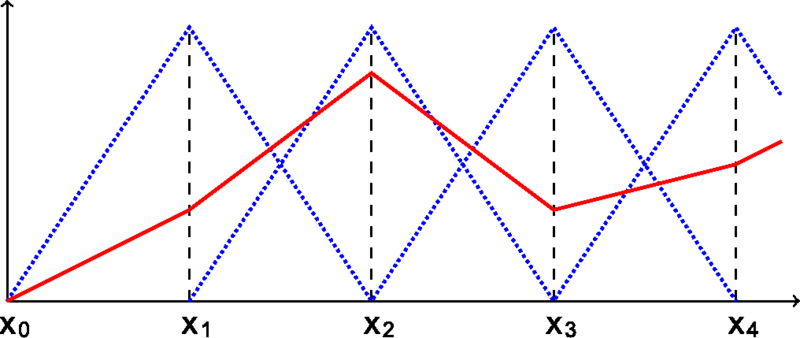
\includegraphics[width=0.75\textwidth]{tent.png}
    \end{figure}
    \end{frame}

    \begin{frame}{Linear B-splines}
    \begin{itemize}
    \item Linear B-splines are \al{piecewise linear} functions.
    \item They are continuous but not differentiable at the knots.
    \item This is simply connecting points with straight lines!
    \item Easy to implement and \alb{shape-preserving}. Easy to evaluate.
\end{itemize}
        \end{frame}    
\end{document}